\documentclass[11pt,a4paper]{article}
\usepackage[T1]{fontenc}
\usepackage[latin1]{inputenc}
\usepackage{lmodern}
\usepackage{float}
\usepackage{a4wide}
\usepackage[dvips]{graphicx}

\usepackage[
pdfauthor={ACE Project Team},
pdftitle={Developers Guide},
pdfcreator={pdftex},
]{hyperref}

\usepackage{sectsty}
\allsectionsfont{\sffamily}

\usepackage{fancyheadings} 
\pagestyle{fancy} 
\lhead{\textsf{\textbf{ACE} \\ \small{a collaborative editor}}}
\chead{}
\rhead{
\parbox[c]{3cm}{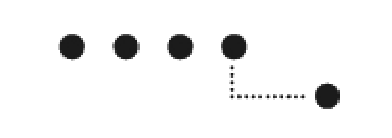
\includegraphics[height=0.875cm,width=3cm]{../../images/logo_BFH.eps}}
\parbox[c]{2.2cm}
{\tiny{\textsf{Berner Fachhochschule \\
Hochschule f�r \\
Technik und Informatik}}}}
\lfoot{}
\cfoot{\textsf{\thepage}}
\rfoot{}
\setlength{\headrulewidth}{0.6pt}
\setlength{\footrulewidth}{0.6pt}
\setlength{\topmargin}{-50pt}
\addtolength{\headheight}{50pt}

\usepackage{colortbl}

\newcommand{\headercol}[2]{\multicolumn{1}{|>{\bfseries\columncolor[gray]{0.82}}p{#1}|}{\textsf{#2}}}
\newcommand{\ace}[0]{\emph{ACE }}



\begin{document}

\setlength{\parindent}{0pt}
\setlength{\parskip}{0pt}

\begin{titlepage}
\thispagestyle{empty}
  
\includegraphics[height=1.5in]{../images/pix.eps}

  \begin{center}

    {\fontsize{40}{45} \textbf{\textsf{ACE}}} \\
    \textsf{a collaborative editor} \\
        
    \vspace{36pt}
        
    {\huge{\textbf{\textsf{}}}} \\

    \vspace{36pt}

	\textsf{Berne University of Applied Sciences} \\
    \textsf{School of Engineering and Information Technology} \\
    
  \end{center}

  \vfill
  
  \begin{tabular}{ll}
   \hline

   \\

   \multicolumn{1}{>{\bfseries}p{1.5in}}{\textsf{Date:}} &
   \multicolumn{1}{>{}p{4.3in}}{\textsf{08.11.2005}}          \\
   
   \\
   
   \multicolumn{1}{>{\bfseries}p{1.5in}}{\textsf{Version:}}     &   
   \multicolumn{1}{>{}p{4.3in}}{\textsf{0.1}}                 \\

   \\
   
   \multicolumn{1}{>{\bfseries}p{1.5in}}{\textsf{Projectteam:}}                 &
   \multicolumn{1}{>{}p{4.3in}}{\textsf{Mark Bigler (biglm2@hta-bi.bfh.ch)}}  \\
   \multicolumn{1}{>{\bfseries}p{1.5in}}{}                                      &
   \multicolumn{1}{>{}p{4.3in}}{\textsf{Simon Raess (rasss@hta-bi.bfh.ch)}}    \\
   \multicolumn{1}{>{\bfseries}p{1.5in}}{}                                      &
   \multicolumn{1}{>{}p{4.3in}}{\textsf{Lukas Zbinden (zbinl@hta-bi.bfh.ch)}} \\   
   
   \\
   
   \multicolumn{1}{>{\bfseries}p{1.5in}}{\textsf{Receivers:}}                       &
   \multicolumn{1}{>{}p{4.3in}}{\textsf{Jean-Paul Dubois (doj@hta-bi.bfh.ch)}}       \\
   \multicolumn{1}{>{\bfseries}p{1.5in}}{}                                          &
   \multicolumn{1}{>{}p{4.3in}}{\textsf{Claude Fuhrer (frc@hta-bi.bfh.ch)}}       \\

   \\
   
   \multicolumn{1}{>{\bfseries}p{1.5in}}{\textsf{Location:}}               &   
   \multicolumn{1}{>{}p{4.3in}}{\textsf{Subversion Repository}} \\

   \\  
   
   \hline
  \end{tabular}

\end{titlepage}


\tableofcontents
\newpage


\section{Introduction}
The \emph{Developers Guide} is intended to show a potential developer what
is needed to develop. It includes the following information:

\begin{itemize}
 \item setting up the development environment
 \item directory structure: what can be found where?
 \item package structure
 \item Ant build file and description of targets
 \item building installers
\end{itemize} 

You find information about how to build, test, and run the application.

\textbf{Note:} Unless you want to change the source code, we do not recommend 
to build the
application from source. We provide installers for Windows and an
application bundle for Mac OS X. These install a completely working
application without the need of building the application from source.


\subsection{Quick Start}
For the impatient among here the steps to execute ACE.

\begin{itemize}
 \item setup the project environment
 \begin{itemize}
  \item install Subversion
  \item install Java SDK 1.4.2 or greater
  \item install Ant 1.6 or greater
  \item install Maven 2.0 Ant tasks
 \end{itemize}
 \item type \texttt{ant run} in the top-level directory of ACE
\end{itemize}

These steps and some additional things are explained in detail in the
following sections.


\subsection{Wiki and Issue Tracker}

\subsubsection{Trac}
In the first stage of the project we used \texttt{trac}, a combined wiki, issue tracker, and repository browser. Trac is still running, but we do not use it anymore as wiki and issue tracker. (\href{http://ace.iserver.ch:81/cgi-bin/trac.cgi}{http://ace.iserver.ch:81/cgi-bin/trac.cgi})

\subsubsection{Jira}
We switched to Jira as our issue tracker. At the moment, this issue tracker is used to keep track of open tasks, bugs, and enhancements. 
(\href{http://ace.iserver.ch:8080/jira}{http://ace.iserver.ch:8080/jira})

\subsubsection{Confluence}
Currently, we use Confluence as our wiki. (\href{http://ace.iserver.ch:8080/confluence}{http://ace.iserver.ch:8080/confluence})



\section{Setup}


\subsection{Subversion}
The complete source of ACE is kept in a Subversion repository. The repository
URL is \href{http://ace.iserver.ch:81/repos/ace/}{http://ace.iserver.ch:81/repos/ace/}. To get the source, you have to install a Subversion client.
There are different pre-packaged binaries available on the Internet.
Select one on the download site of Subversion
(\href{http://subversion.tigris.org/}{http://subversion.tigris.org/})
or install it from source. You should install at least Subversion 1.1.x,
because we store symbolic links in the repository, which are only supported
since Subversion 1.1.


\subsection{Java J2SE SDK}
ACE is programmed with Java 1.4.2. So, if you have not installed the
Java J2SE SDK download it from the Sun Java website 
(\href{http://java.sun.com/j2se/}{http://java.sun.com/j2se/}). Note,
any version greater or equal than 1.4.2 should be fine.


\subsection{Apache Ant}
ACE uses Apache Ant (see \href{http://ant.apache.org/}{http://ant.apache.org/})
to build the application. If you have not installed Ant, download and install
it from the above URL. We recomment that you download the latest stable
version of Ant. At the time of writing this is \texttt{1.6.5}.
Further, we use a special Ant task to download the
dependency jar files used by ACE. 
These libraries are not stored in the Subversion repository.


\subsection{Maven 2.0 Ant Tasks}
Maven 2.0 now comes with a set of Ant tasks that can be used to use Maven's
artifact handling features from within Ant. This includes most notably the
\emph{transitive dependency management} of Maven 2.0. You can
download these Ant tasks from \\
\href{http://maven.apache.org/download.html}{http://maven.apache.org/download.html}.

\subsubsection{Installation}
To install the Maven Ant tasks you have to do the following:
\begin{itemize}
 \item download the maven-artifact-ant-2.0-dep.jar from the Maven download site
 \item copy the downloaded jar file to the directory \texttt{ANTHOME/lib} where \texttt{ANTHOME} is where Ant is installed
\end{itemize}

\subsubsection{Maven Repositories}
ACE uses two different Maven repositories. A Maven repository is a place where
dependencies are installed. The first repository is a custom repository that
stores all dependencies that are not available from the default Maven
repository. The URL of this repository is http://ace.iserver.ch/maven2. The
second repository is the standard Maven repository at the URL
http://repo1.maven.org/maven2/.

\subsubsection{Dependencies}
In the \texttt{build.xml} you find the declaration of the dependencies.

\small{
\begin{verbatim}
<artifact:dependencies pathId="dependency.classpath">
		<dependency groupId="jdom" 
		            artifactId="jdom" 
		            version="1.0"/>
		<dependency groupId="commons-beanutils" 
		            artifactId="commons-beanutils" 
		            version="1.7.0"/>
        ...
</artifact:dependencies>
\end{verbatim}
}

A dependency has a group id, an artifact id, and a version. You have to know
these in order to add dependencies (browse the Maven repositories in the
web browser to find out the correct values). 
The dependencies are downloaded to a local repository,
which can be found in the user's home directory in the folder 
\texttt{.m2/repository/}.

The id given to the set of dependencies with the \texttt{pathId} attribute
can be used like any other path in the Ant build file. The Maven Ant tasks
allow to get the correct versions of dependencies without needing to place
them in the source repository.

To find out more about the Maven Ant tasks visit
\href{http://maven.apache.org/ant-tasks.html}{http://maven.apache.org/ant-tasks.html}.

\subsubsection{First Time Build}
When you run the build the first time you will get a couple of messages saying that dependencies are downloaded to the local maven repository. You will get 
some warnings too, because the task first checks the custom
repository of ACE, which does not contain all the dependencies of the project.


\subsection{Bonjour}
ACE uses Bonjour (see \href{http://www.apple.com/macosx/features/bonjour/}{http://www.apple.com/macosx/features/bonjour/}) for its discovery features.
As Bonjour uses native code, you need to install some platform 
dependent code.

\subsubsection{Mac OS X}
Nothing needs to be installed because the required libraries are installed
by default.

\subsubsection{Windows}
If you have installed iTunes on your computer, Bonjour for Windows is
already installed. Otherwise you need to get it from the above URL.

\subsubsection{Posix}
Unfortunately, there is no installer for Bonjour on Posix Operating Systems
(at least to our knowledge).
That means, you have to build Bonjour from source. In the following instructions, replace os=linux with your operating system. Check the Makefile in \texttt{mDNSPosix/Makefile} for supported operating systems.

\begin{itemize}
 \item download the source code from here
 \item unpack the downloaded tar.gz to a location of your choice
 \item go to the subdirectory \texttt{mDNSPosix}
 \item in the Makefile, adjust the variable JDK to point to the correct JDK location
 \item type \texttt{make os=linux} to build the \texttt{mDNSResponder}
 \item as root user, type \texttt{make os=linux install} to install the \texttt{mDNSResponder} daemon
 \item now, the daemon needs to be started by running the startup script \texttt{/etc/init.d/mdns start} as root
\end{itemize}

Further, you have to build a shared library in order that Bonjour for Java works:

\begin{itemize}
 \item in the directory \texttt{mDNSPosix} type \texttt{make os=linux Java}
 \item as root, copy the file \texttt{libjdns\_sd.so} from \texttt{build/prod} to somewhere into the Java library path (system property \texttt{java.library.path})
\end{itemize}


\subsection{Latex}
If you want to build the documentation you need to install \LaTeX{}.



\section{Directory Structure}
ACE has the following contents in the top-level directory:

\begin{itemize}
 \item \texttt{build}: the build directory
 \item \texttt{build.xml}: the main build file
 \item \texttt{dist}: distributions
 \item \texttt{doc}: documentation
 \item \texttt{LICENSE.txt}: ACE project license
 \item \texttt{project.properties}: properties used by Maven
 \item \texttt{project.xml}: Maven project.xml
 \item \texttt{src}: the sources of the project
 \item \texttt{www}: the project website
\end{itemize}


\subsection{Build Products}
The \texttt{build} folder contains the build results of the project:

\begin{itemize}
 \item \texttt{ant-graph.*}: dependency graph of Ant build file
 \item \texttt{api}: generated javadoc API documentation
 \item \texttt{build-dependencies.xml}: generated build file to copy dependencies
 \item \texttt{classes}: compiled classes from src/java
 \item \texttt{integration-test}: compiled classes from src/integration-test
 \item \texttt{lib}: copied dependency jar files
 \item \texttt{osx}: compiled classes from src/osx as well as the application bundle
 \item \texttt{resources}: copied resources from src/resources
 \item \texttt{resources-test}: copied resources from src/resources-test
 \item \texttt{stubs}: compiled classes from src/stub
 \item \texttt{test}: compiled classes from src/test
 \item \texttt{testreports}: JUnit testreports
\end{itemize}


\subsection{Sources}
The \texttt{src} folder contains the sources of the project.

\begin{itemize}
 \item \texttt{installer}: windows NSIS installer scripts
 \item \texttt{integration-test}: integration tests
 \item \texttt{java}: java sources
 \item \texttt{osx}: OS X customization java code and template for application bundle
 \item \texttt{resources}: runtime resources (images, property files, ...)
 \item \texttt{resources-test}: test resources
 \item \texttt{stubs}: stub classes for testing purpose
 \item \texttt{test}: JUnit tests
 \item \texttt{test-app}: test applications
\end{itemize}


\subsection{Documentation}
The \texttt{doc} folder contains the sources of the project:

\begin{itemize}
 \item \texttt{developersguide}: the \LaTeX{} sources of the developers guide
 \item \texttt{finalreport}: thd \LaTeX{} sources of the final report
 \item \texttt{images}: images for the documentation
 \item \texttt{latex}: \LaTeX{} templates
 \item \texttt{projectmanual}: the \LaTeX{} sources of the project manual
 \item \texttt{systemrequirements}: the \LaTeX{} sources of the system requirements
 \item \texttt{templates}: source code header
 \item \texttt{usermanual}: the \LaTeX{} sources of the user manual
\end{itemize}



\section{Package Structure}
ACE has the following package structure:

\begin{itemize}
 \item \texttt{ch.iserver.ace} - top level package
 \item \texttt{ch.iserver.ace.algorithm} and its subpackages - all algorithm related classes and interfaces
 \item \texttt{ch.iserver.ace.application} and its subpackages - the implementation of the application layer
 \item \texttt{ch.iserver.ace.collaboration} - the interfaces of the API between the application and the collaboration layer
 \item \texttt{ch.iserver.ace.collaboration.jupiter} and its subpackages - implementation of the collaboration layer using \emph{Jupiter}
 \item \texttt{ch.iserver.ace.net} - the interfaces of the API between the collaboration and the network layer
 \item \texttt{ch.iserver.ace.net.*} and its subpackages - implementation of the network layer
 \item \texttt{ch.iserver.ace.util} and its subpackages - utility classes used by several packages (includes the implementation of the thread domain concept)
\end{itemize}



\section{Build File}

\begin{figure}[H]
 \centering
 \includegraphics[width=15cm,height=19.84cm]{../images/developersguide/ant-graph.eps}
 \caption{Ant build file dependencies}
\end{figure}

The main targets are:
\begin{itemize}
 \item \texttt{compile}
 \item \texttt{test}
 \item \texttt{integration-test}
 \item \texttt{run}
 \item \texttt{clean}
 \item \texttt{javadoc}
 \item \texttt{dist}
\end{itemize}


\subsection{Compiling the Sources}
To compile the sources you use the Ant target \texttt{compile}. 


\subsection{Running the Tests}
There are two test targets. The first that runs the unit tests is called
\texttt{test}. These tests are run regularly by our continous integration
server. The test sources are found in the directory \texttt{/src/test}. They
must run quickly and deterministically.

The other test target is \texttt{integration-test} which runs integration tests.
Integration tests test large parts of the system and thus run slower than
the pure unit tests.


\subsection{Running the Application}
You can run the application by calling the \texttt{run} target, which starts
the main class of the whole application. If you want to run another class
with a main method, you can start it with by calling the \texttt{run-class}
task with a system property \texttt{class} set to the correct class name.
You do this from the command line with an additional argument 
\texttt{-Dclass=...}. To debug the application, there is a \texttt{debug}
target that starts the JVM with the correct startup parameters. Connect
your favorite debugger to the JVM. The connection parameters are:
\begin{itemize}
 \item connection type: socket attach
 \item host: localhost
 \item port: 8000
\end{itemize}


\subsection{Cleaning the Build Results}
The \texttt{clean} target can be used to clean the build directory,
forcing a complete rebuild.


\subsection{Javadoc}
The \texttt{javadoc} target creates the Javadoc API of the application into the
directory \texttt{/build/api}.


\subsection{Creating a Distribution}
The Ant target \texttt{dist} creates a \texttt{tar.gz} file containing the
sources, the javadoc, and all the necessary jar files into the directory
\texttt{/dist}. Further it builds some the Mac OS X application bundle if
you run that target on an OS X machine.



\section{Installers}
The build file has some targets to create OS specific installers. Currently,
there are installers for OS X and Windows.


\subsection{OS X}
The OS X installer is built by the target \texttt{dist-osx}, which is 
called by the standard \texttt{dist} target. The \texttt{dist-osx} target
does not have all the necessary dependencies declared. Normally, you should
just invoke \texttt{dist} to build the whole distribution (including
the OS X installer). 

The OS X installer can only
be built on OS X for two reasons. First, the targets use a command line
utility only available on OS X and second, the customization Java code
for OS X relies on Apple Java extensions, which are not available on
other systems.

The resulting disk image is placed in the \texttt{dist} folder. The disk
image can be mounted on Mac OS X. The disk image contains
the application bundle.

\subsubsection{Application Bundles}
On Mac OS X, an application is basically a folder containing a specialized
structure, called application bundle. The extension of such an application
bundle is \texttt{.app}. A bundle has the following basic content:

\begin{figure}[H]
 \centering
 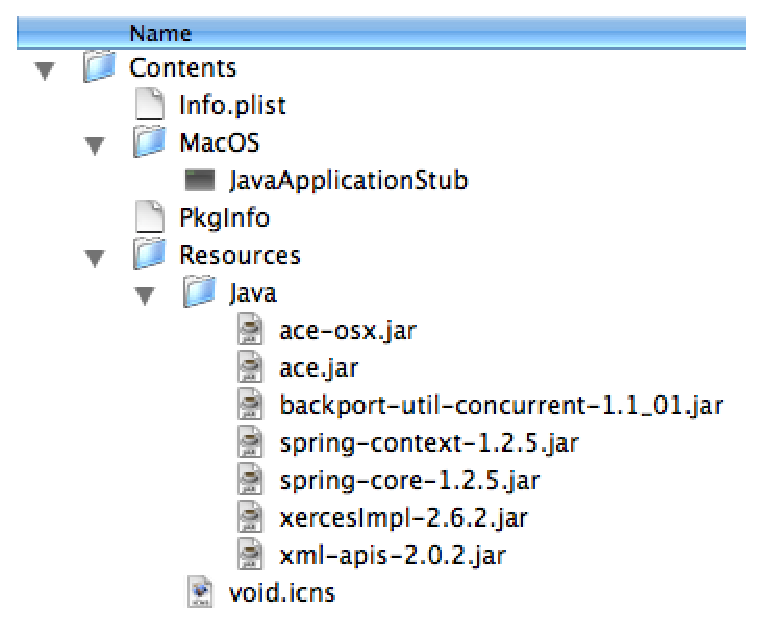
\includegraphics[width=12.3cm,height=10.2cm]{../images/developersguide/app-bundle.eps}
 \caption{application bundle structure}
\end{figure}

The file \texttt{Info.plist} is used by the operating system to determine
things like the executable, the icons for the application, Java version to
use, and the classpath. The \texttt{Resources} folder contains all the
resources needed by the application. In ACE, all the required jar files
are placed inside a subfolder of \texttt{Resources}.

Application bundles can be installed by simply moving the bundle into any
place the user likes. There is no need for an installer. Everything needed
by the application is contained in the bundle. Launching the application
happens by double-clicking the application bundle.

\subsubsection{Ant Targets}
The Ant targets ending with \texttt{osx} are used to build the Mac OS X
application bundle. Before calling them you should first call the following
targets:

\begin{itemize}
 \item \texttt{jar}
 \item \texttt{copy-dependencies}
\end{itemize}

The OS X build requires a custom Ant task called \texttt{EnhancerTask}. 
This task determines all the needed
dependency libraries from a fileset. It allows further to exclude some
unwanted dependencies, for instance JUnit libraries, by specifying excludes.
This task is needed because we define dependencies as Maven Ant task
dependencies. A dependency can have additional dependencies, which in turn
can have dependencies, and so on. The dependency declaration from 
the Maven Ant task allows to set a \texttt{fileset} attribute, which allows to
get all the needed dependency jar files.

The task enhances the classpath of a skeleton \texttt{Info.plist} file with all
the dependencies of ACE. It must be defined with a \texttt{typedef}:
\small{
\begin{verbatim}
<typedef name="enhance"
         classname="ch.iserver.ace.ant.dependency.EnhancerTask"
         classpathref="enhancer.classpath"/>
\end{verbatim}
}

The enhance task can have two attributes.
\begin{itemize}
 \item \texttt{source}: the source \texttt{Info.plist} file
 \item \texttt{target}: the generated enhanced \texttt{Info.plist} file
\end{itemize}

Further, the enhance task supports nested \texttt{fileset} elements as well
as \texttt{exclude} elements. All the files included by the fileset are
added to the classpath declaration in the \texttt{Info.plist} file, except
for those files that are explicitely excluded by an exclude element.

\small{
\begin{verbatim}
<enhance source="Info.plist" target="Info.plist.enhanced">
  <fileset refid="dependency.fileset"/>
  <exclude name="junit*.jar"/>
</enhance>
\end{verbatim}
}


\subsection{Windows}
The ACE-Installer for windows is based on \textit{Nullsoft Scriptable Install System (NSIS)} (\href{http://nsis.sf.net/}{http://nsis.sf.net/}). Two scripts named \texttt{MakeACELauncherJavaw.nsi} and \texttt{MakeACEInstaller.nsi} are needed to build the windows installer executable. Both can be found in \texttt{src/windows/installer} in the ACE source repository.

Compile the nsis-script's either in the console with the command:
\begin{verbatim}
[...]src\windows\installer>makensis.exe SCRIPT_NAME.nsis
\end{verbatim}
or start \texttt{makensisw.exe} and drag \& drop your files onto it.

\begin{description}
\item[Step 1:] Build all jar files and copy them into the library folder in your installer directory. Use the following steps:
  \begin{itemize}
  \item Make a new library folder in your installer directory called \texttt{lib}.
  \item Run the ant-targets \texttt{ant dist} and \texttt{ant dist-windows}.
  \item Copy all files from the \texttt{build/lib} into the created library folder.
  \end{itemize}

\item[Step 2:] Make the \texttt{ACE.exe} executable. Open the nsis-scipt \texttt{MakeACELauncherJavaw.nsi} in a simple text editor and add all libraries to the classpath variable. Further, check that the class variable has the correct value:
\begin{verbatim}
  !define CLASSPATH "lib\lib-1.jar; lib\lib-2.jar; ... "
  
  !define CLASS "ch.iserver.ace.application.Main"
\end{verbatim}

\item[Step 3:] Make the \texttt{ACEInstaller.exe} executable. Open the nsis-script \texttt{MakeACEInstaller.nsi} in a simple text editor and add all libraries to the install section. Note: you do not have to put them into the uninstall section too because uninstall will delete the whole library folder automatically.
\begin{verbatim}
Section "Install" InstallSection
[...]

File "lib\lib-1.jar"
File "lib\lib-2.jar"
File "lib\ ... "
\end{verbatim}

\end{description}


\end{document}
